\chapter{Lec 11 - NP-Hardness}

\section{Tractable vs Intractable problems}
Problems for which a polynomial algorithm exists are called \textbf{tractable}. If no such algorithm exists, the problem is called \textbf{intractable}.\newline\newline
\textbf{Examples:}
\begin{enumerate}
    \item \textbf{Eulerian circuit problem:} Given an undirected graph, an Eulerian circuit is a cycle that traverses all the edges only once. This problem can be solved in linear time. Note that in an Euler circuit you might pass through a vertex more than once.

    \item \textbf{Hamiltonian circuit problem:} Given an undirected graph, an Hamiltonian circuit is a cycle that traverses all the vertices only once. To date, no one knows a polynomial algorithm to solve it. Note that in a Hamiltonian circuit you may not pass through all edges.

    \item \textbf{Minimum spanning tree:}

    \item \textbf{Traveling Salesperson Problem (TSP):} Given a complete, undirected graph and a function $w: E \rightarrow \mathbb{R}$, output a \textbf{tour} (i.e. a cycle that visits every vertex exactly once) of minimum cost
    \[T \subseteq E \quad \text{minimizing }\sum_{e \in T}w(e)\]
    To date, no one knows a polynomial algorithm to solve it.
\end{enumerate}
A much easier task can be the following: Given a graph and a list of vertices $C$, \textbf{check} if $C$ is an Hamiltonian circuit.\newline\newline
Problems that are \textit{easy} to solve belong to the \textbf{complexity class} \textbf{P} (\textit{polynomial time}), 1), 3) $\in$ \textbf{P}. Problems that are \textit{easy} to verify belong to the complexity class \textbf{NP} (\textit{Non-deterministic polynomial}), 1), 2) ,3) ,4) $\in$ \textbf{NP}.

\section{NP-Hard}
\textbf{Decision Problems:}\newline
To simplify the study of the complexity of problems, we limit our attention to problems with a boolean answer (YES, NO), that is, decision problems.\newline\newline
Let's define \textbf{P} and \textbf{NP} classes in a more formal way:
\begin{itemize}
    \item \textbf{P} is the set of decision problems that can be solved in polynomial time.

    \item \textbf{NP} is the set of decision problems with the following property: if the answer is YES, then there is a proof of this fact that can be checked in polynomial time.

    \item \textbf{NP-Hard:} A computational problem is \textbf{NP-Hard} if a polynomial-time algorithm that solves it would imply a polynomial-time algorithm that solves every problem in \textbf{NP}.\newline\newline
    A problem is \textbf{NP-Complete} if it is both in \textbf{NP} and \textbf{NP-Hard}. Basically, these problems are the hardest in \textbf{NP}. 
\end{itemize}
\begin{figure}[h]
    \centering
    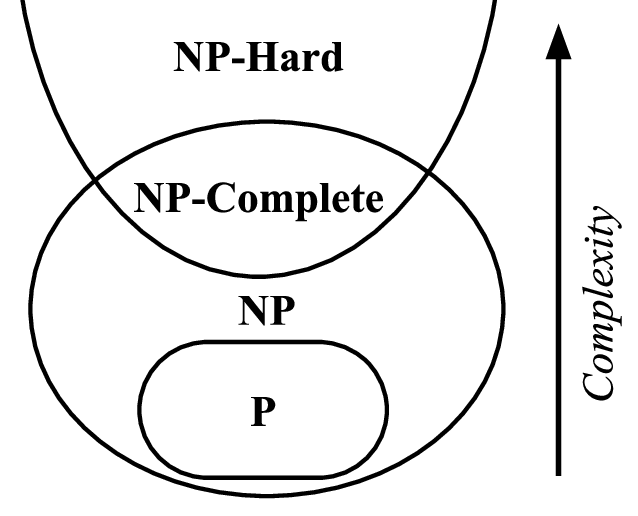
\includegraphics[scale=0.4]{images/P-NP.png}
    \caption{What we think the computation classes look like}
    \label{fig:P-NP-Np-Hard}
\end{figure}
One of the main open questions in computer science is whether \textbf{P=NP}.\newline\newline
Studying NP-Hardness is important because if a problem is \textbf{NP-Hard} is a strong evidence that it is intractable. It suggests you to use a different approach, such as identify tractable special-cases, or use \textbf{approximation algorithms}.

\section{Cook-Levin Theorem}
\textit{In computational complexity theory, the Cook–Levin theorem, also known as Cook's theorem, states that the Boolean satisfiability problem is \textbf{NP-complete}.}\footnote{Wikipedia definition}\newline\newline
SAT: formula satisfiability:
\begin{itemize}
    \item input: A boolean formula like the following: $(b \land \neg c) \lor (\neg a \land b)$

    \item output: It is possible to assign boolean values to the variables $a, b, c, ...$ such that the entire formula evaluates to TRUE?
\end{itemize}
determining the satisfiability of a formula in conjunctive normal form (CNF) where each clause is limited to at most three literals is \textbf{NP-complete} also; this problem is called \textbf{3-SAT}.\newline\newline
\textbf{Example of 3-CNF formula:}
\[(a \lor b \lor c) \land (b \lor \neg c \lor \neg d) \land (\neg a \lor c \lor d)\]
%Check if the theorem was defined on 3SAT???
How can we show that a problem is \textbf{NP-Hard}?

\section{Reductions}

To prove that a problem $P$ is \textbf{NP-Hard} we use \textbf{reduction}. We want to prove that every problem in \textbf{NP} reduces to problem $P$.\newline\newline
Reducing problem $A$ to problem $B$ means describing an algorithm to solve $A$ under the assumption that an algorithm for $B$ exists.
\begin{center}
    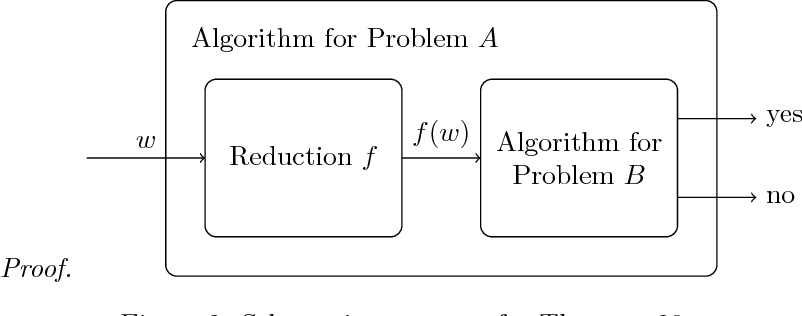
\includegraphics[scale=0.4]{images/Reduction.png}
\end{center}
$A < B$ means \textit{A reduces to B} where $B$ is the hardest problem ($A$ is as hard as $B$).

